\documentclass[11pt,spanish,a4paper]{article}
% Versión 1.er cuat 2021 Víctor Bettachini < bettachini@df.uba.ar >

% Versión 1.er cuat 2021 Víctor Bettachini < bettachini@df.uba.ar >

\usepackage[T1]{fontenc}
\usepackage[utf8]{inputenc}

\usepackage[spanish, es-tabla]{babel}
\def\spanishoptions{argentina} % Was macht dass?
% \usepackage{babelbib}
% \selectbiblanguage{spanish}
% \addto\shorthandsspanish{\spanishdeactivate{~<>}}

\usepackage{graphicx}
\graphicspath{{./figuras/}}
% \usepackage{float}

\usepackage[arrowdel]{physics}
\newcommand{\pvec}[1]{\vec{#1}\mkern2mu\vphantom{#1}}
% \usepackage{units}
\usepackage[separate-uncertainty=true, multi-part-units=single, locale=FR]{siunitx}
\usepackage{isotope} % $\isotope[A][Z]{X}\to\isotope[A-4][Z-2]{Y}+\isotope[4][2]{\alpha}

\usepackage{tasks}
\usepackage[inline]{enumitem}
% \usepackage{enumerate}

\usepackage{hyperref}

% \usepackage{amsmath}
% \usepackage{amstext}
\usepackage{amssymb}

\usepackage{tikz}
\usepackage{tikz-dimline}
\usetikzlibrary{math}
\usetikzlibrary{arrows.meta}
% \usetikzlibrary{snakes}
% \usetikzlibrary{calc}
\usetikzlibrary{decorations.pathmorphing}
\usetikzlibrary{patterns}

\usepackage[hmargin=1cm,vmargin=1.6cm,nohead]{geometry}
% \voffset-3.5cm
% \hoffset-3cm
% \setlength{\textwidth}{17.5cm}
% \setlength{\textheight}{27cm}

\usepackage{lastpage}
\usepackage{fancyhdr}
\pagestyle{fancyplain}
\fancyhead{}
\fancyfoot{{\tiny \textcopyright DF, FCEyN, UBA}}
\fancyfoot[C]{ {\tiny Actualizado al \today} }
\fancyfoot[RO, LE]{Pág. \thepage/\pageref{LastPage}}
\renewcommand{\headrulewidth}{0pt}
\renewcommand{\footrulewidth}{0pt}


\begin{document}
\begin{center}
	\textbf{Física 2} (Físicos) \hfill \textcopyright {\tt DF, FCEyN, UBA}\\
	\textsc{\LARGE Láminas retardadoras}
\end{center}

Los ejercicios con (*) entrañan una dificultad adicional. Son para investigar después de resolver los demás.


\begin{enumerate}

\section*{Láminas retardadoras o de onda}

\item Se hace incidir luz circularmente polarizada en sentido horario sobre una lámina retardadora de cuarto de onda ($+\lambda/4$).
¿Cuál es el estado de polarización de la luz al emerger de la misma?



\item Sobre una lámina de cuarto de onda incide un haz de luz natural de intensidad $I_0$.
¿Con qué estado de polarización emerge?
¿Cuál es su intensidad?
Justifique.



\item Incide luz plano polarizada sobre una lámina de cuarto de onda.
El plano de polarización es paralelo al eje óptico de la misma.
¿Cuál es el estado de polarización de la luz que emerge de la lámina?



\item Una onda linealmente polarizada incide sobre una lámina de media onda ($+\lambda/2$).
El plano de polarización forma un ángulo de \ang{30;;} con el eje óptico de la lámina (considere que el eje óptico es el eje rápido).
¿Cuál es el estado de polarización de la luz que sale de la misma?



\item Incide luz elípticamente polarizada en sentido antihorario sobre una lámina de cuarto de onda.
A medida que se va rotando la lámina retardadora, ¿cuál es el estado de polarización de la luz que emerge?



\item Sobre una lámina de cuarto de onda incide normalmente una vibración monocromática elípticamente polarizada.
Las componentes $E_x$ y $E_y$ del vector campo eléctrico están relacionadas por:
\[
	\frac{ E_x^2 }{ 9 } \pm \frac{ \sqrt{ 2 } }{ 12 } E_x E_y + \frac{ E_y^2 }{ 16 } = \frac{ 1 }{ 2 }
\]
Considere que $x$ es el eje óptico de la lámina, y que dicho eje es el rápido.
\begin{enumerate}
	\item Hallar el estado de polarización de dicha vibración a la salida de la lámina.
	\item Se coloca detrás de la lámina un polarizador cuyo eje óptico forma \ang{30;;} con el eje óptico de la lámina.
	Hallar la vibración que abandona el polarizador, ¿cuál es el porcentaje de energía perdido en la lámina y cuál en el polarizador?
\end{enumerate}

\section*{Analizador: láminas + polarizador}

\item ¿Cómo puede hacerse para analizar luz elípticamente polarizada?


\item ¿Cuál es la diferencia que existe entre luz parcialmente polarizada y luz elípticamente polarizada?
¿Cómo se puede hacer para distinguirlas?



\item Se tienen dos fuentes luminosas: i) una de luz natural, y ii) otra que consiste en la superposición de luz natural con una onda monocromática de una longitud de onda $\lambda$ conocida, circularmente polarizada.
¿Cómo puede Ud. saber cuál es i) y cuál es ii)?
Para ello Ud. dispone de polaroids, láminas de media onda y láminas de cuarto de onda (todos los que quiera).
Especifique claramente qué elementos utilizaría para distinguirlas y justifique.



\item Un alumno de Laboratorio 2 necesita utilizar una fuente de luz circularmente polarizada derecha lo más potente posible.
Sin embargo, sólo dispone de una fuente de luz elípticamente polarizada izquierda tal que el eje mayor de la perturbación es cuatro veces el eje menor.
Además dispone de los siguientes elementos: i) dos láminas iguales de cuarto de onda y ii) un polaroid.
\begin{enumerate}
	\item Establezca, justificando claramente su elección, los elementos que utilizaría, en qué orden, y con qué objetivos, para lograr la fuente que necesita.
	No olvide que se quiere que la fuente sea lo más potente posible.
	\item Elija un sistema de coordenadas, y en un plano perpendicular a la dirección de propagación dibuje la evolución temporal de la perturbación incidente.
	Escriba el vector que representa a dicha perturbación.
	\item Calcule el ángulo que los ejes de cada elemento deben formar con los ejes propios de la perturbación incidente y el ángulo que los ejes propios de la perturbación emergente de cada elemento forman con los ejes propios de la perturbación incidente.
\end{enumerate}



\item Se tiene un haz de luz monocromática linealmente polarizada y se desea diseñar un dispositivo que logre rotar el vector campo eléctrico a \ang{90;;} del inicial, de forma tal que la intensidad a la salida sea aproximadamente la misma que a la entrada.
Para armar dicho dispositivo usted dispone de láminas de cuarto de onda y polaroids.
\begin{enumerate}
	\item Diga qué elementos usaría, en qué orden y con qué objetivos.
	\item Calcule los ángulos entre los ejes propios de cada elemento y la dirección del campo incidente y la polarización del campo eléctrico a la salida de cada elemento.
	\item ¿Podría lograr el mismo objetivo si en lugar de disponer de láminas de cuarto de onda y polaroids, dispusiera de láminas de media onda y polaroids?
	De ser así, ¿qué elementos usaría?
	Justifique claramente su respuesta.
\end{enumerate}



\item Se tiene un haz de luz monocromática y linealmente polarizada.
A partir de ella se desea obtener luz elípticamente polarizada en sentido antihorario, mediante una lámina de \(\lambda/4\).
Se desea que el eje mayor de la elipse sea tres veces el eje menor.
Hallar el ángulo que debe formar el plano de polarización de la luz incidente con el eje rápido de la lámina para que el campo eléctrico a la salida de la lámina
tenga la polarización pedida (si más de un valor es posible, alcanza con que dé uno de ellos).
¿Cuáles son los ejes de la elipse?



\item Se tiene un dispositivo compuesto por una fuente que emite luz de frecuencias $\omega_1$ y $\omega_2$, un polarizador y dos láminas retardadoras de idénticas características.
Cada una de éstas se comporta como lámina de cuarto de onda para la luz incidente de frecuencia $\omega_1$ y como lámina de media onda para la frecuencia $\omega_2$.
\begin{enumerate}
	\item ¿Que relación deben cumplir $\omega_1$ y $\omega_2$ para que las láminas retardadoras puedan tener la propiedad mencionada? \medskip{} \\
	La luz emitida por la fuente incide sobre el polarizador; el eje de transmisión del mismo tiene una dirección conocida.
	Seguidamente al polarizador se coloca una de las láminas retardadoras con su eje rápido formando un ángulo de \ang{+30;;} respecto del eje de transmisión del polarizador.
	A continuación se ubica la segunda lámina con su eje rápido formando un ángulo de \ang{+30;;} respecto del eje rápido de la primera lámina (es decir, a \ang{+60;;} del eje de transmisión del polarizador).
	\item Escriba la amplitud del campo eléctrico a la salida de cada elemento (lámina o polarizador) para ambas frecuencias.
	Indique el tipo de polarización que se tiene en cada caso. 
\end{enumerate}



\item
\begin{minipage}[t][4cm]{0.55\textwidth}
Se tiene una interfase plana entre aire y vidrio ($n = \num{1.5}$).
A cierta distancia de la misma, se coloca una fuente que emite una onda monocromática.
Dicha onda se propaga en la dirección $z$, está elípticamente polarizada en sentido antihorario, siendo su eje mayor tres veces el eje menor, e incide sobre la interfase luego de atravesar una lámina de \(\lambda/4\) (ver figuras).
La lámina de \(\lambda/4\) puede girarse, lo mismo que la fuente.
Se desea que no haya onda reflejada.
\end{minipage}
\begin{minipage}[c][-1cm][t]{0.4\textwidth}
	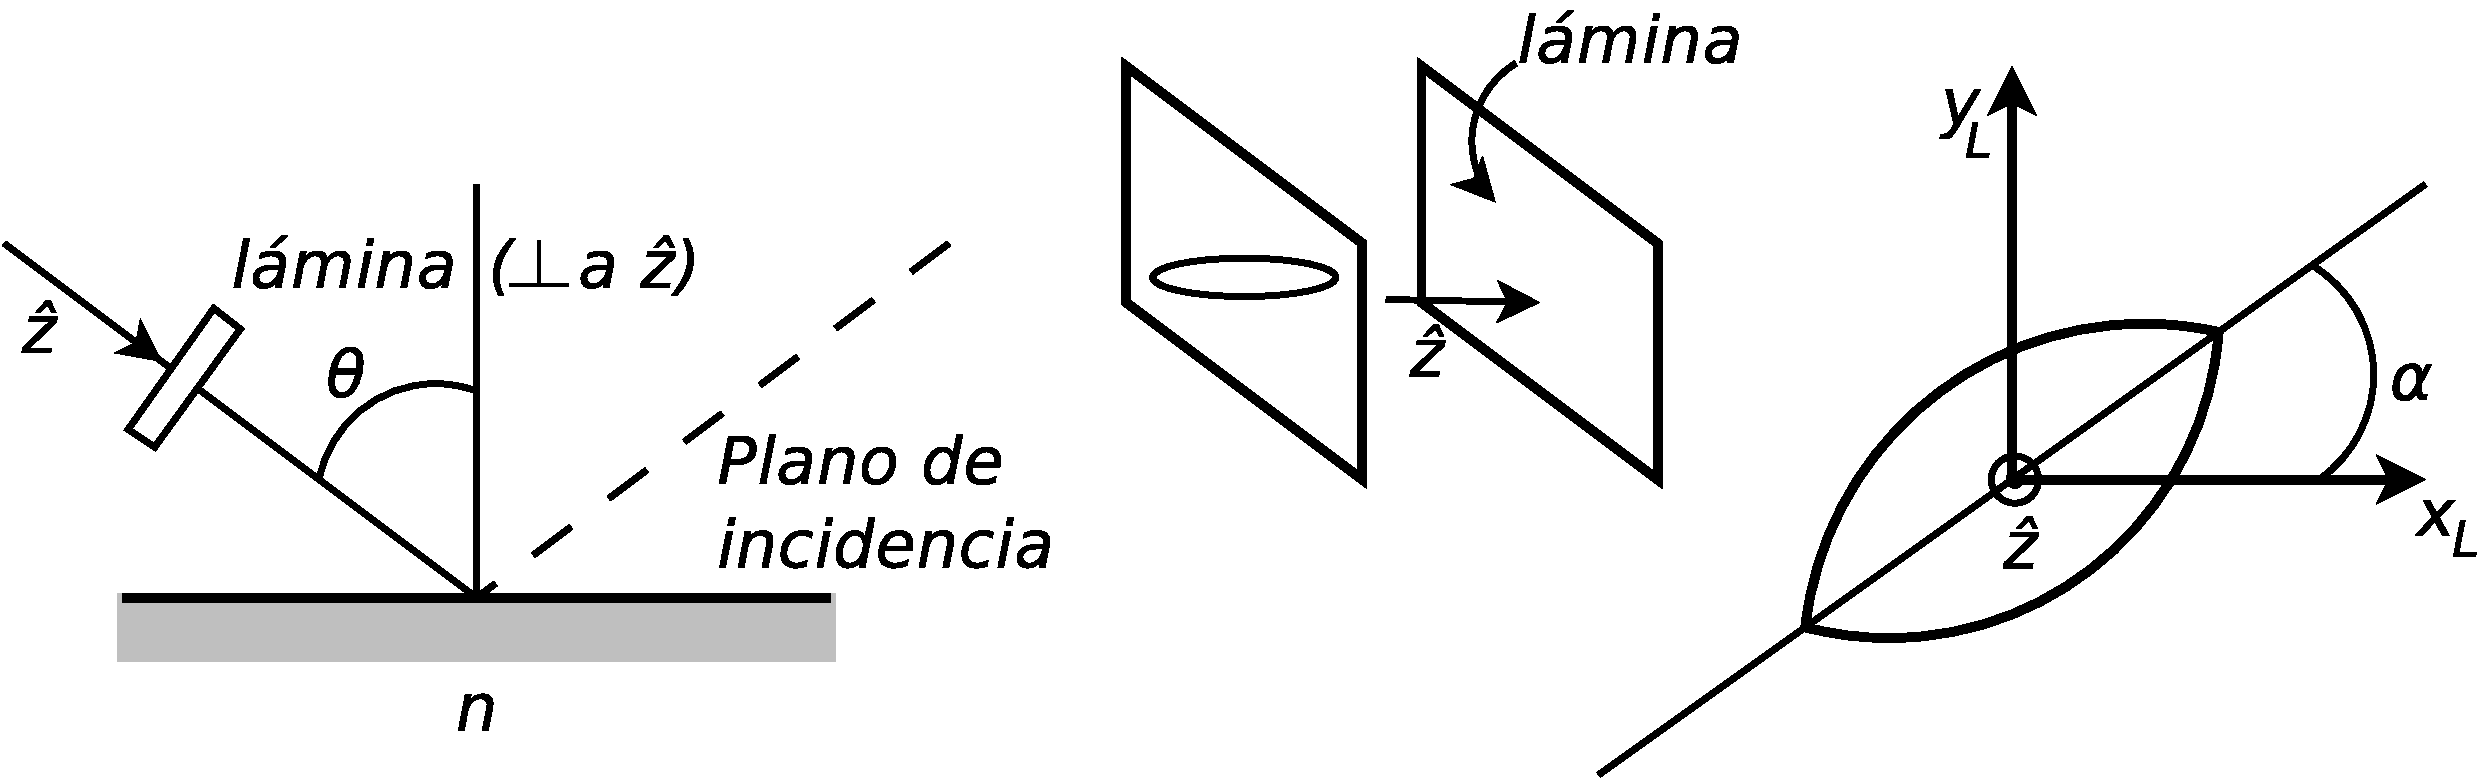
\includegraphics[width=\textwidth]{ej4-28}
\end{minipage}
\begin{enumerate}
	\item ¿Cuál debería ser la polarización del campo a la salida de la lámina para que esto sea factible?
	Teniendo esto en cuenta:
	\item Diga cómo debe orientarse la fuente con respecto a los ejes de la lámina.
	Es decir, halle cuál debe ser el ángulo $\alpha$ formado entre el eje mayor de la elipse y el eje rápido de la lámina ($x_{L}$).
	Halle el campo a la salida de la lámina.
	\begin{itemize}
		\item halle el ángulo de incidencia ($\theta$)
		\item halle el ángulo que debe formar el eje $y_L$ de la lámina con la dirección perpendicular al plano de incidencia. 
	\end{itemize}
\end{enumerate}
Sugerencia: escriba \textbf{claramente} la expresión del campo eléctrico a la entrada y a la salida de la lámina, indicando el o los sistemas de coordenadas que usa.



\end{enumerate}

\end{document}
